\chapter{The \lhcb detector}
\label{sec:Detector}

Most parts of this chapter are taken from \cite{detector}

The \lhcb experiment is one of the four big experiments, currently running at the Large Hadron Collider (LHC) of the European Organization for Nuclear Research CERN in Geneva, Switzerland. In contrast to the other three experiments -- \atlas and \cms are searching for direct hints of new physics, \alice investigates the Quark-Gluon-Plasma -- \lhcb is dedicated to look indirectly for physics beyond the Standard Model (see section \ref{sec:Theory}) by the study of hadrons containing either a heavy \bquark- or \cquark-quark.

...

The layout of the \lhcb detector can be seen in figure \ref{fig:detector}. It is built as a single-arm forward spectrometer. The reason for this choice is, that at \lhc energies of $\sqs = 14 \tev$ at the maximum, \bquark- and \bquarkbar- hadrons are predominantly produced in the forward (or backward) region.

\begin{figure}[hptb]
    \centering
	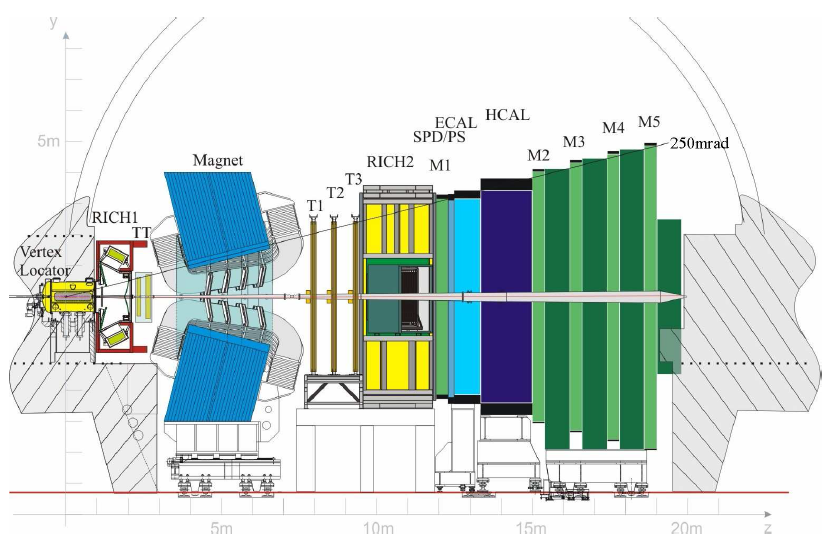
\includegraphics[width=\textwidth]{lhcb-detector}	
	\caption{The \lhcb detector.}
	\label{fig:detector}
\end{figure}

% ===========================
% SECTION: Tracking detectors
% ===========================
\section{Tracking detectors}
Tracking describes the whole procedure to reconstruct the trajectories of the (charged) particles produced in the proton-proton collision. If there's a magnet in use, the particles' charges and momenta can be determined as well. For that purpose, a system of several subdetectors is aligned up- and downstream the dipole magnet, namely the Vertex locator (VELO), the Trigger Tracker (TT) and the Trigger stations (T1-T3) built-up by the Inner Tracker (IT) and the Outer Tracker (OT).

\subsection{Vertex Locator (VELO)}
The VErtex LOcator (VELO) is placed directly around the primary interaction point. 
Its task is to precisely measure the track coordinates of charged particles and separate the proton-proton interaction point from other vertices, namely either other primary vertices (so called pile-up events) or secondary vertices. 
The latter ones are typically for \bquark- or \cquark-hadron decays \cite{VELO_TDR} and a good separation and resolution of these vertices is crucial for the \lhcb physics programme.
As an example serves the measurement of particles' decay length and time for the determination of the rapid $\Bs-\Bsb$ oscillation frequency \cite{BsBsbar_frequency}.

The VELO is built up by silicon modules due to the high particle flux and thus high radiation in the interaction region. It is placed only 7\mm apart from the beam. This is closer than the required aperture of the \lhcb beam pipe at injection. Thus, the VELO sensors are made of silicon microstrips shaped as slightly overlapping half-discs. The two halfs can be moved in $x$- and $y$-direction to avoid radiation damages unless the beam is stable.

Each module provides a measurement of the $r$- and $\phi$-coordinates.
The sensores for these measurements are correspondingly called $R$- and $\Phi$-sensor, which can be seen in figure \ref{fig:VELO_RandPhiSensor}.
An overview over the VELO system with its modules is shown in figure \ref{fig:VELO_Overview}. Around the nominal interaction region, the modules are placed closer to each other. Upstream there are two $R$ sensors dedicated to veto pile-up events. 
Figure \ref{fig:VELO_Overview} furthermore shows the VELO in closed and opened position.
\begin{figure}[hptb]
    \centering
	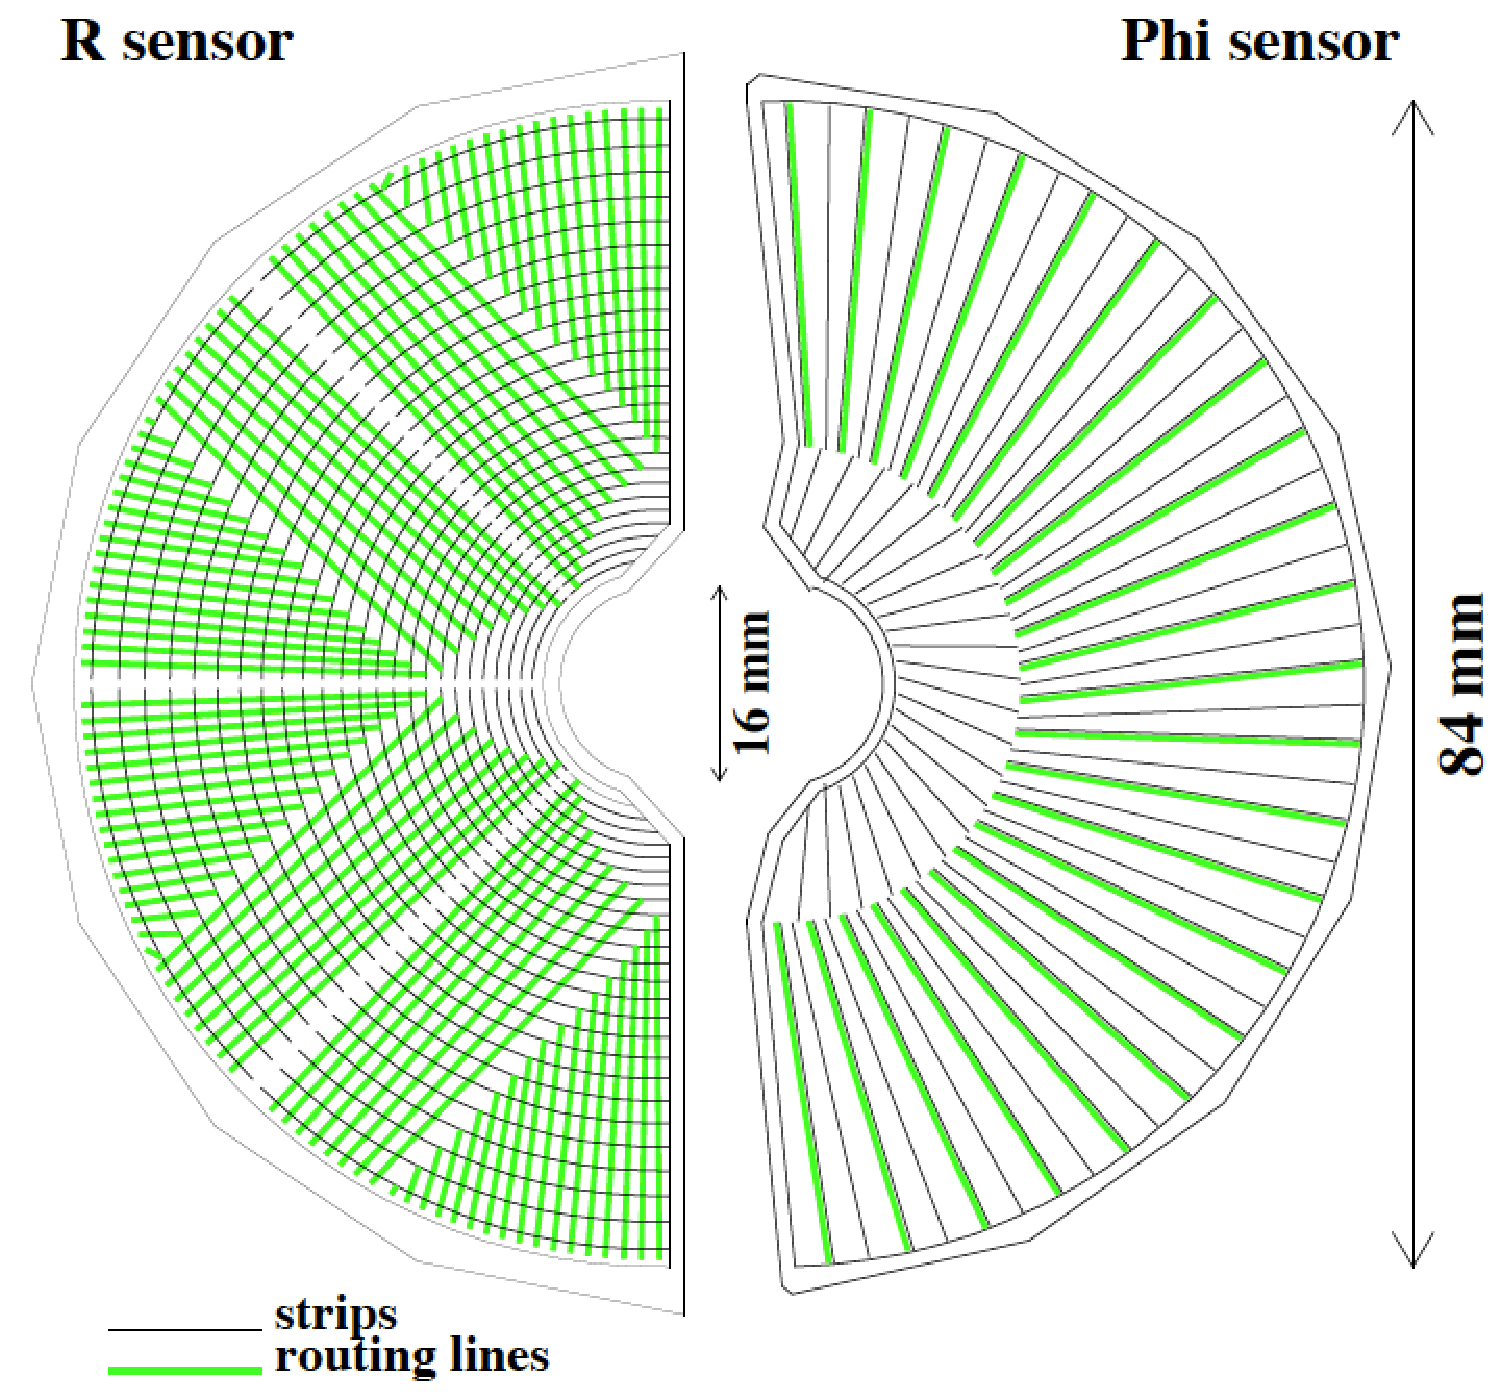
\includegraphics[width=0.5\textwidth]{VELO_randphisensors}	
	\caption{Schematic representation of an $R$ and a $\Phi$ sensor. The $R$ sensor strips are arranged into four approximately 45\degrees segments and have routing lines perpendicular to the strips. The $\Phi$ sensor has two zones with inner and outer strips. The routing lines of the inner strips
    are orientated parallel to the outer strips. Figure and caption taken from \cite{VELO_Performance}.}
	\label{fig:VELO_RandPhiSensor}
\end{figure}
\begin{figure}[hptb]
    \centering
	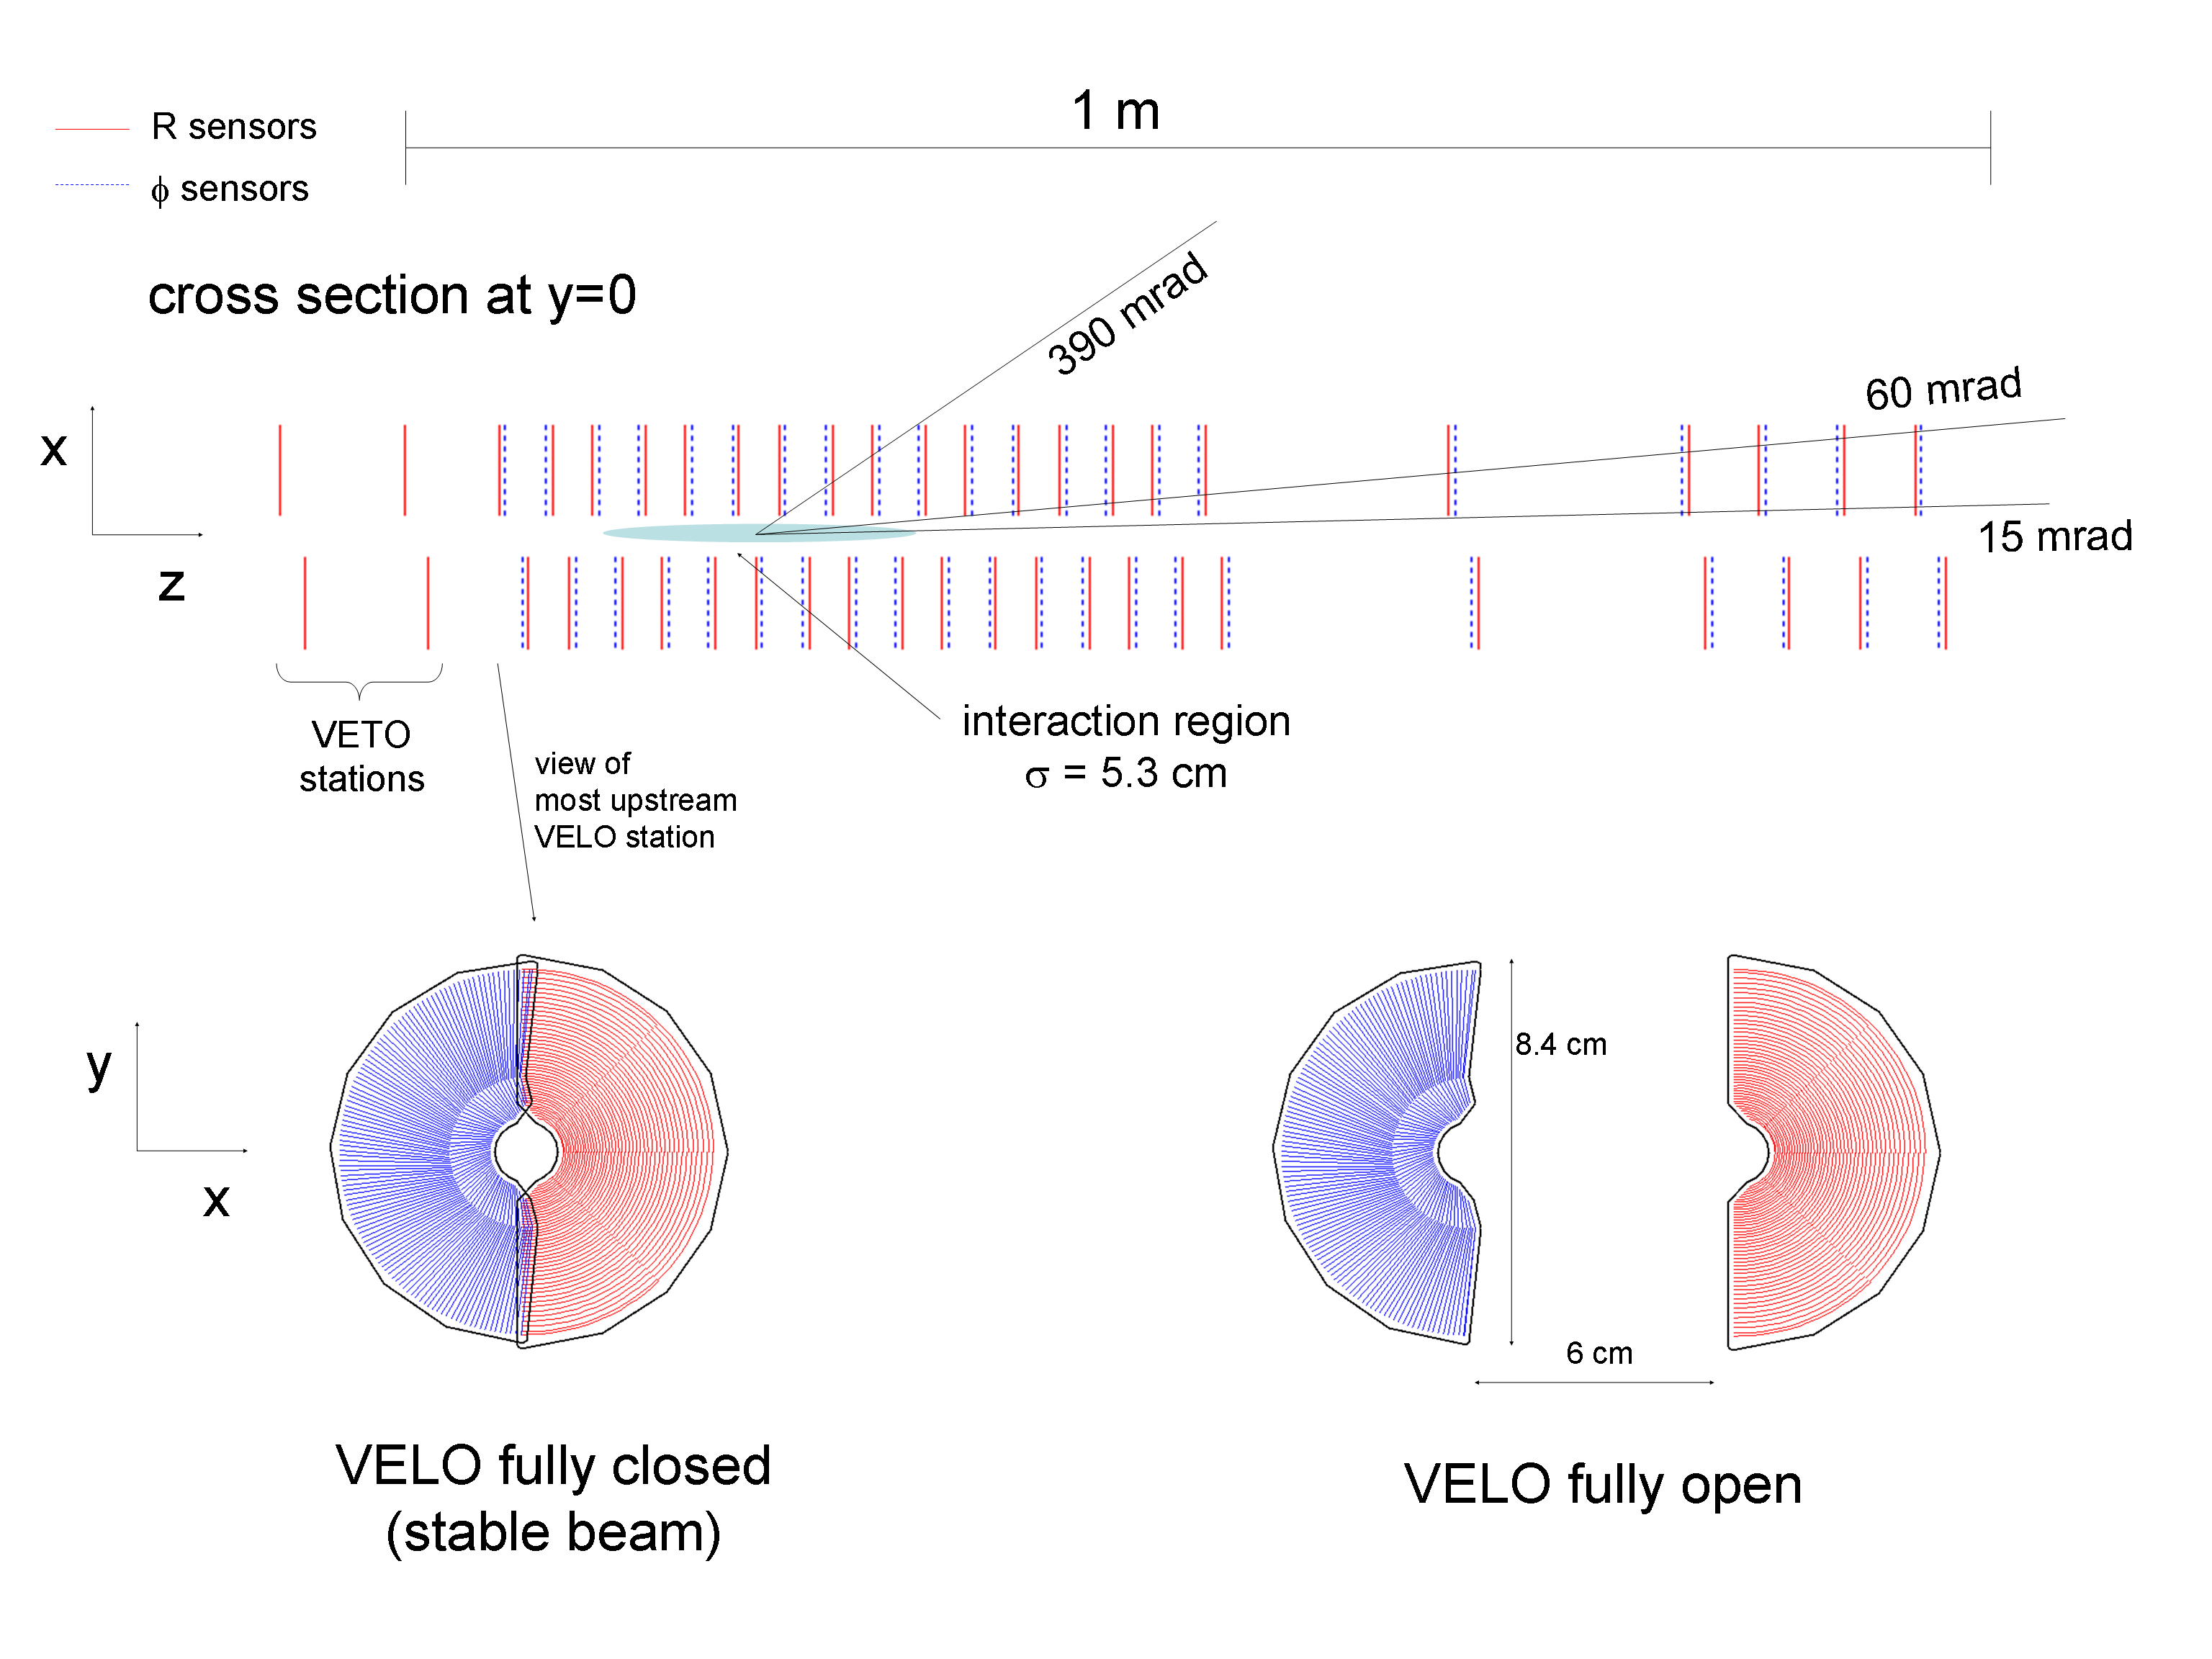
\includegraphics[width=0.8\textwidth]{VELO_Overview}	
	\caption{Cross section in the $(x,z)$ plane of the VELO silicon sensors, at $y=0$, with the detector in the fully closed position. 
             The front face of the first modules is also illustrated in both the closed and open positions. 
             The two pile-up veto stations are located upstream of the VELO sensors.
             Figure and caption taken from \cite{detector}.}
	\label{fig:VELO_Overview}
\end{figure}
With this setup the VELO reaches a track finding efficiency above 98\%. Its resolution on vertices is 13\mum in the transverse plane and 71\mum along the beam axis for vertices with 25 tracks. 
The resolution on the impact parameter is smaller than 35\mum for particles with a transverse momentum larger than 1\gev \cite{detector, VELO_TDR, VELO_Performance}.

\subsection{Trigger Tracker / Tracker Turicensis (TT)}
The Tracker Turicencis or formerly the Trigger Tracker is located in front of the entrance of the \lhcb magnet. It is used for sevaral tasks:
\begin{itemize}
    \item deliver transverse momentum information for Level-1 trigger,
    \item reconstruct trajectories of long-lived neutral particles decaying outside the VELO
    \item reconstruct low-momenta particles bent out by the magnet before reaching the station T1-T3.
\end{itemize}

The TT makes completely use of silicon microstrip detector. It consist of one station made of four planes along the beam axis. The first and the fourth layer have vertical readout strips ($x$-layer), while the second and third are rotated by an angle $\pm 5\degrees$ to get a high resolution in the
bending plane and additional information in $y$-direction.
Between the $u$ and $v$ layer there is a gap of around 30\cm. Figure \ref{fig:TT_layers} shows schematically the layout of the TT.
\begin{figure}[hptb]
    \centering
	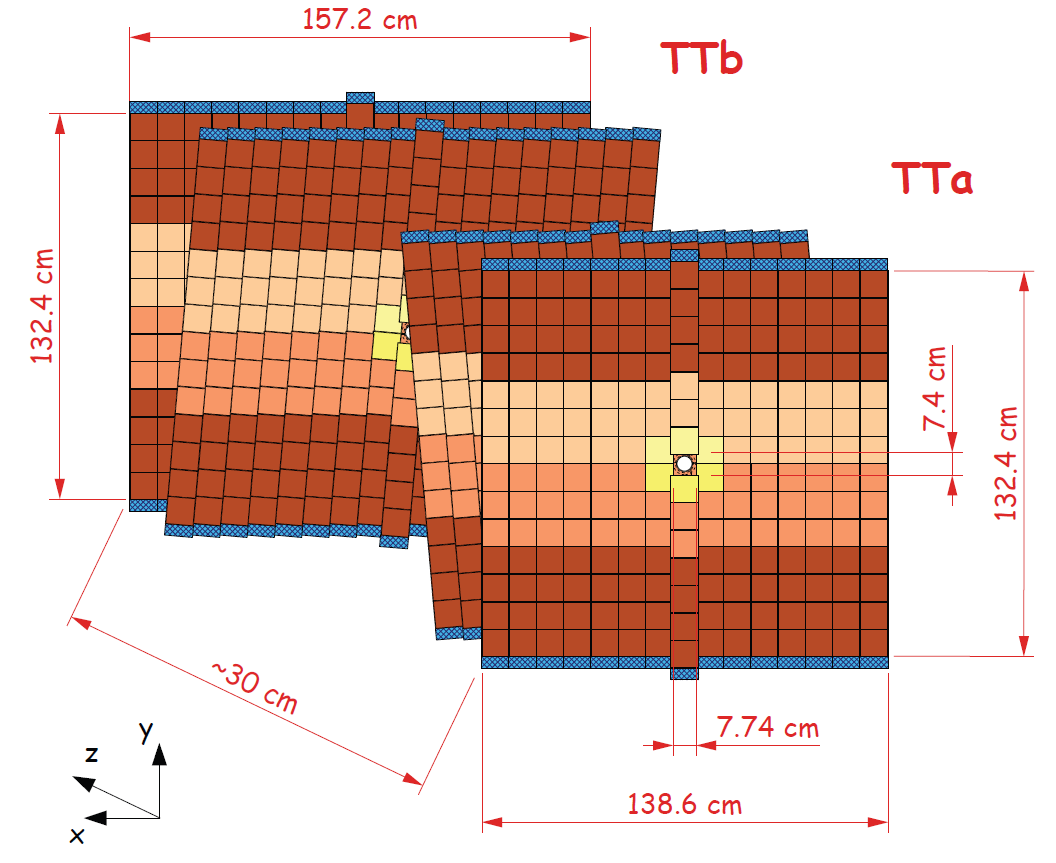
\includegraphics[width=0.8\textwidth]{TT_layers}	
	\caption{Layout of the Tracker Turicensis (TT). 
             Figure taken from \cite{ST_Performance}.}
	\label{fig:TT_layers}
\end{figure}

\subsection{Inner Tracker (IT)}
Being a silicon micro-strip detector, the Inner Tracker (IT) uses the same technology as the TT. 
It builds the inner part of the three tracking stations T1-T3 (see figure \ref{fig:detector}).
Each station consists of four boxes as shown in figure \ref{fig:IT_layer}.
In each box there are again 4 layers, two vertical and two stereo, analogously to the TT \cite{detector, ST_Performance}.
\begin{figure}[hptb]
    \centering
	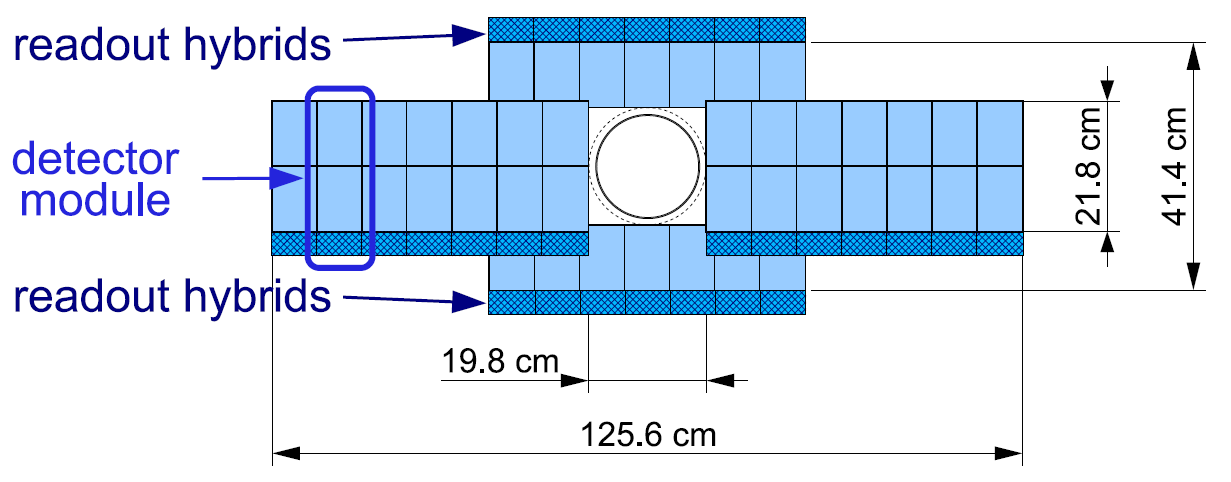
\includegraphics[width=0.8\textwidth]{IT_layer}	
	\caption{Layout of a $x$ detection layer in the second Inner Tracker (IT) station. 
             Figure taken from \cite{detector}.}
	\label{fig:IT_layer}
\end{figure}

\subsection{Outer Tracker (OT)}

\subsection{Track classification}


% ================================
% SECTION: Particle identification
% ================================
\section{Particle identification}

\subsection{Ring Imaging Cherenkoy Detector (RICH)}

\subsection{Calorimeter system}

\subsection{Muon chambers}

% ===========================
% SECTION: Trigger
% ===========================
\section{Trigger}

\subsection{L0-Trigger}

\subsection{High Level Trigger (HLT)}
